\documentclass{article}\usepackage{graphicx, color}
%% maxwidth is the original width if it is less than linewidth
%% otherwise use linewidth (to make sure the graphics do not exceed the margin)
\makeatletter
\def\maxwidth{ %
  \ifdim\Gin@nat@width>\linewidth
    \linewidth
  \else
    \Gin@nat@width
  \fi
}
\makeatother

\usepackage{Sweavel}



\usepackage{microtype}
\usepackage[utf8]{inputenc}
\usepackage[T1]{fontenc}
\usepackage{amsmath}
\usepackage{mathpazo}
\usepackage{siunitx}
\usepackage{listings}
\usepackage{minted}
\usepackage{inconsolata}
\usepackage{caption}
\captionsetup{skip=0pt,labelfont=bf}
\lstset{breaklines=true,showstringspaces=false}
\newcommand{\Rstat}{\textsf{R}}




\begin{document}
The data is saved in a file named \texttt{baguiorainfall.dat}. We input this data in \Rstat{} and define a variable \texttt{baguiorainseries} using the \texttt{ts} function.

\begin{Schunk}
\begin{Sinput}
baguiorain <- read.table("baguiorainfall.dat")
baguiorainseries <- ts(baguiorain, frequency = 12, start = c(2001, 1))
\end{Sinput}
\end{Schunk}


Figure \eqref{fig:TSPlot} shows the graph of the rain fall time series from January 2001 to December 2011. We can see that the data is seasonal, peaking every July to August every year.

\begin{figure}[!ht]
\centering
\begin{Schunk}
\begin{Sinput}
plot.ts(baguiorainseries)
\end{Sinput}

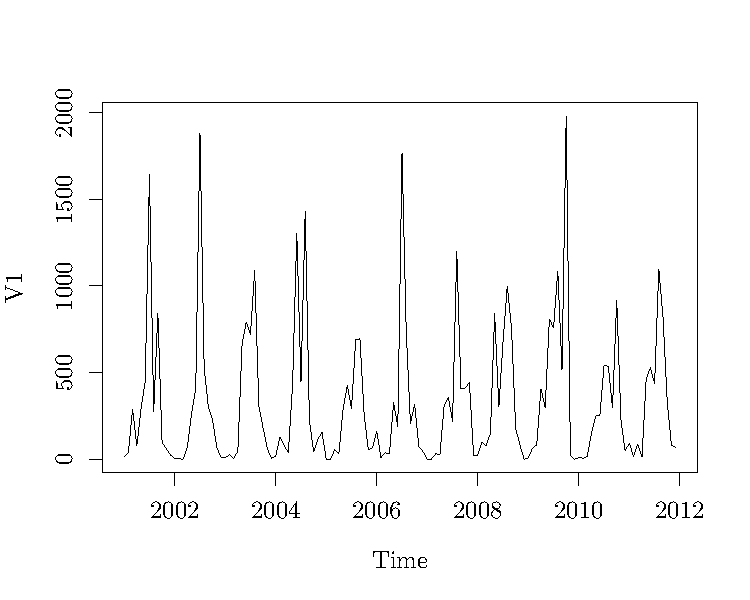
\includegraphics[width=.7\textwidth]{figure/listings-YeastBoxPlot} \end{Schunk}


\caption{\label{fig:TSPlot} Plot of Baguio rain fall time series, from January 2001 to December 2011.}
\end{figure}

Here, the time series data is broken down into its components. This is done in preparation to eliminating the seasonal component of the data.

\begin{center}
\begin{Schunk}
\begin{Sinput}
baguiorainseriescomponents <- decompose(baguiorainseries)
baguiorainseriescomponents
\end{Sinput}
\begin{Soutput}
$x
          Jan      Feb      Mar      Apr      May      Jun      Jul
2001   14.600   39.500  289.800   76.000  291.000  451.400 1642.000
2002    5.000    2.000    0.600   71.200  264.400  411.000 1883.400
2003    9.800   25.400    4.800   46.800  662.700  792.400  721.300
2004   17.000  128.600   79.870   37.800  428.600 1306.500  445.400
2005    0.200    0.000   54.600   32.000  291.000  425.700  292.400
2006  160.600    8.800   38.400   29.600  327.509  188.200 1769.800
2007    0.000    0.600   31.800   25.400  308.600  358.400  219.000
2008   24.000   97.000   78.700  149.800  839.800  302.000  681.200
2009    8.000   64.500   82.900  407.300  298.500  810.000  758.400
2010   10.037    5.499   15.300  148.600  248.600  254.000  543.700
2011   94.000   13.800   88.900   11.900  462.500  529.100  435.900
          Aug      Sep      Oct      Nov      Dec
2001  274.000  842.200   97.000   61.600   23.200
2002  525.600  301.500  224.800   67.300   10.000
2003 1089.400  303.200  179.700   60.400    4.400
2004 1432.900  225.600   42.400  114.500  154.900
2005  690.200  694.600  256.600   55.200   68.000
2006  735.800  207.600  316.000   72.400   43.200
2007 1201.600  408.400  410.300  444.800   21.600
2008  999.500  761.000  178.100   82.600    0.000
2009 1087.700  516.900 1981.800   22.200    0.000
2010  536.600  296.800  920.100  226.400   47.400
2011 1096.300  819.200  332.400   81.600   67.400

$seasonal
         Jan     Feb     Mar     Apr     May     Jun     Jul     Aug
2001 -296.55 -293.19 -283.56 -235.99   80.13  204.37  561.21  522.65
2002 -296.55 -293.19 -283.56 -235.99   80.13  204.37  561.21  522.65
2003 -296.55 -293.19 -283.56 -235.99   80.13  204.37  561.21  522.65
2004 -296.55 -293.19 -283.56 -235.99   80.13  204.37  561.21  522.65
2005 -296.55 -293.19 -283.56 -235.99   80.13  204.37  561.21  522.65
2006 -296.55 -293.19 -283.56 -235.99   80.13  204.37  561.21  522.65
2007 -296.55 -293.19 -283.56 -235.99   80.13  204.37  561.21  522.65
2008 -296.55 -293.19 -283.56 -235.99   80.13  204.37  561.21  522.65
2009 -296.55 -293.19 -283.56 -235.99   80.13  204.37  561.21  522.65
2010 -296.55 -293.19 -283.56 -235.99   80.13  204.37  561.21  522.65
2011 -296.55 -293.19 -283.56 -235.99   80.13  204.37  561.21  522.65
         Sep     Oct     Nov     Dec
2001  122.05  128.05 -212.33 -296.84
2002  122.05  128.05 -212.33 -296.84
2003  122.05  128.05 -212.33 -296.84
2004  122.05  128.05 -212.33 -296.84
2005  122.05  128.05 -212.33 -296.84
2006  122.05  128.05 -212.33 -296.84
2007  122.05  128.05 -212.33 -296.84
2008  122.05  128.05 -212.33 -296.84
2009  122.05  128.05 -212.33 -296.84
2010  122.05  128.05 -212.33 -296.84
2011  122.05  128.05 -212.33 -296.84

$trend
       Jan   Feb   Mar   Apr   May   Jun   Jul   Aug   Sep   Oct   Nov
2001    NA    NA    NA    NA    NA    NA 341.5 339.5 325.9 313.6 312.3
2002 317.9 338.4 326.4 309.2 314.8 314.4 314.1 315.3 316.4 315.6 331.2
2003 331.1 306.2 329.8 327.9 325.8 325.3 325.3 329.9 337.4 340.1 330.0
2004 351.6 354.4 365.5 356.5 353.0 361.6 367.1 361.1 354.7 353.4 347.4
2005 261.9 224.6 213.2 241.6 248.1 242.0 245.1 252.1 251.8 251.0 252.4
2006 295.7 359.2 340.8 323.0 326.2 325.9 318.1 311.1 310.5 310.0 309.1
2007 257.8 212.6 240.4 252.7 272.2 286.8 286.9 291.9 297.9 305.0 332.3
2008 369.0 379.8 386.1 391.1 366.4 350.4 348.8 346.8 345.6 356.5 344.7
2009 367.7 374.6 368.1 433.1 505.7 503.2 503.3 500.9 495.6 482.0 469.2
2010 411.8 379.9 347.8 294.4 258.6 269.1 274.6 278.4 281.8 279.2 282.4
2011 309.8 328.6 373.7 371.0 340.4 335.2    NA    NA    NA    NA    NA
       Dec
2001 309.5
2002 363.7
2003 341.6
2004 305.0
2005 244.1
2006 315.4
2007 352.1
2008 343.3
2009 443.9
2010 302.8
2011    NA

$random
          Jan      Feb      Mar      Apr      May      Jun      Jul
2001       NA       NA       NA       NA       NA       NA  739.334
2002  -16.360  -43.257  -42.248   -2.012 -130.491 -107.820 1008.092
2003  -24.773   12.401  -41.398  -45.158  256.792  262.771 -165.233
2004  -38.020   67.408   -2.038  -82.722   -4.572  740.561 -482.947
2005   34.856   68.622  124.989   26.355  -37.216  -20.666 -513.866
2006  161.414  -57.200  -18.845  -57.396  -78.796 -342.030  890.458
2007   38.698   81.151   74.939    8.675  -43.687 -132.745 -629.083
2008  -48.460   10.347  -23.861   -5.345  393.305 -252.745 -228.816
2009  -63.135  -16.882   -1.623  210.225 -287.329  102.446 -306.076
2010 -105.222  -81.207  -48.910   90.231  -90.157 -219.482 -292.093
2011   80.773  -21.612   -1.236 -123.083   41.921  -10.520       NA
          Aug      Sep      Oct      Nov      Dec
2001 -588.150  394.268 -344.686  -38.390   10.510
2002 -312.329 -136.973 -218.836  -51.528  -56.807
2003  236.821 -156.201 -288.458  -57.242  -40.400
2004  549.165 -251.118 -439.028  -20.565  146.777
2005  -84.563  320.752 -122.478   15.089  120.772
2006  -97.955 -224.932 -122.087  -24.336   24.668
2007  387.054  -11.511  -22.753  324.818  -33.657
2008  130.058  293.343 -306.465  -49.753  -46.457
2009   64.151 -100.768 1371.724 -234.631 -147.076
2010 -264.483 -107.090  512.835  156.306   41.439
2011       NA       NA       NA       NA       NA

$figure
 [1] -296.55 -293.19 -283.56 -235.99   80.13  204.37  561.21  522.65
 [9]  122.05  128.05 -212.33 -296.84

$type
[1] "additive"

attr(,"class")
[1] "decomposed.ts"
\end{Soutput}
\end{Schunk}

\captionof{figure}{\label{fig:Components} The seasonal, trend, and random components.}
\end{center}

It can be seen in Figure \eqref{fig:Components} that the data is of additive type. The plot is in Figure \eqref{fig:ComponentsPlot}. 

\begin{figure}[!ht]
\centering
\begin{Schunk}
\begin{Sinput}
plot(baguiorainseriescomponents)
\end{Sinput}

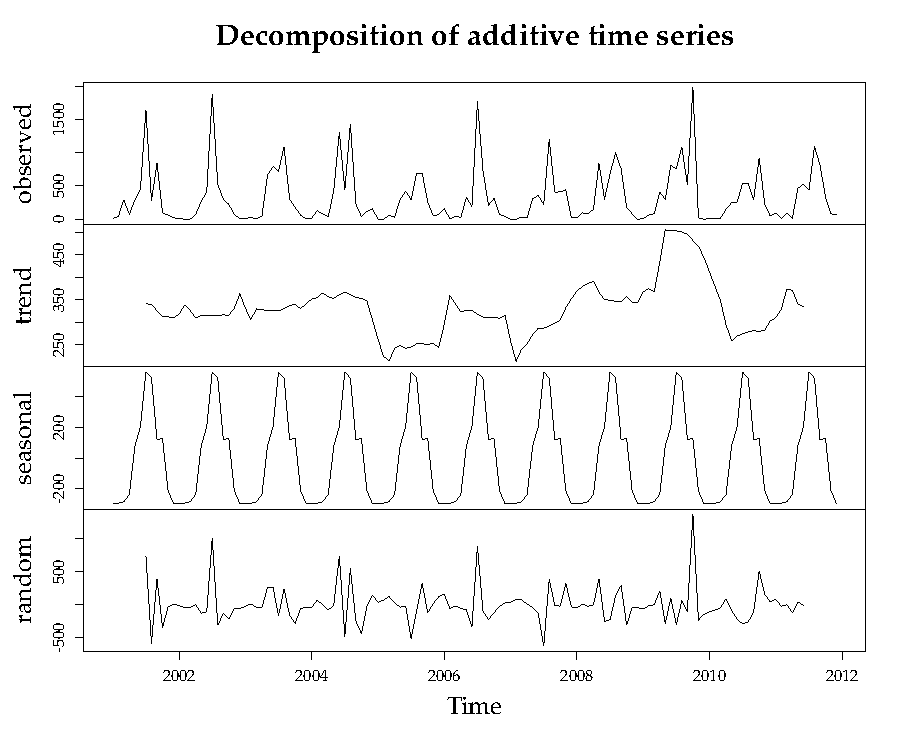
\includegraphics[width=.7\textwidth]{figure/listings-ComponentsPlot} \end{Schunk}


\caption{\label{fig:ComponentsPlot} The plot of the components of the rainfall time series data.}
\end{figure}

To use simple exponential smoothing to make forecasts for the time series of monthly rainfall in Baguio City, we submit the data for Holt-Winters smoothing.

\begin{figure}[!ht]
\begin{Schunk}
\begin{Sinput}
baguiorainseriesforecasts <- HoltWinters(baguiorainseries)
baguiorainseriesforecasts
\end{Sinput}
\begin{Soutput}
Holt-Winters exponential smoothing with trend and additive seasonal component.

Call:
 HoltWinters(x = baguiorainseries) 

Smoothing parameters:
 alpha:  0.001826 
 beta :  0.422 
 gamma:  0.3554 

Coefficients:
         [,1]
a    267.1477
b      0.5062
s1  -208.3311
s2  -227.2503
s3  -194.1851
s4  -136.7234
s5   147.8871
s6   216.3476
s7   338.7154
s8   673.8567
s9   321.0458
s10  430.4775
s11 -130.6776
s12 -215.8636
\end{Soutput}
\end{Schunk}

\caption{\label{fig:HoltWSmoothing} The result of \texttt{Holt Winters} Smoothing.}
\end{figure}

The output of \texttt{HoltWinters()} makes forecast for the same time period covered by the original time series, the time series included rainfall for Baguio City for the period January 2000 to December 2011. So the forecasts are also for that period. An $\alpha$ close to 0 tells us that the forecasts are based on both recent and less recent observations--although somewhat more weight is placed on recent observations (Coghlan 2011). An $\alpha$ of $0.5069$ means that the data can be optimized further to get better prediction. We can eliminate the seasonal trend in order to create a better prediction. The graph of the original time series forecast can be seen in Figure \eqref{fig:ForecastFigure}.

The output of \texttt{HoltWinters()} function is stored in the variable\newline \texttt{baguiorainseriesforecasts\$fitted}. The forecast for the period January 2000 to December 2011 is seen in Figure \eqref{fig:fitted}.

\begin{center}
\begin{Schunk}
\begin{Sinput}
baguiorainseriesforecasts$fitted
\end{Sinput}
\begin{Soutput}
             xhat level     trend   season
Jan 2002   32.503 333.0 -1.698849 -298.800
Feb 2002    7.191 331.3 -1.720038 -322.341
Mar 2002   16.103 329.5 -1.724037 -311.695
Apr 2002  102.143 327.8 -1.735982 -223.891
May 2002  287.964 326.0 -1.759821  -36.254
Jun 2002  433.056 324.2 -1.777976  110.659
Jul 2002 1635.212 322.4 -1.794969 1314.650
Aug 2002  268.024 321.0 -1.603755  -51.387
Sep 2002  848.901 319.9 -1.405308  530.425
Oct 2002  113.125 317.5 -1.827048 -202.525
Nov 2002   77.496 315.9 -1.741009 -236.616
Dec 2002   40.120 314.1 -1.748864 -272.225
Jan 2003    1.962 312.3 -1.772070 -308.556
Feb 2003  -15.416 310.5 -1.766032 -324.183
Mar 2003  -10.089 308.8 -1.734585 -317.195
Apr 2003   70.542 307.1 -1.723114 -234.868
May 2003  259.013 305.4 -1.741406  -44.613
Jun 2003  405.767 304.4 -1.430389  102.835
Jul 2003 1705.198 303.6 -1.132512 1402.692
Aug 2003  338.804 300.7 -1.890546   39.985
Sep 2003  635.117 300.2 -1.312257  336.240
Oct 2003  133.794 298.3 -1.567979 -162.909
Nov 2003   55.021 296.8 -1.532611 -240.233
Dec 2003   10.826 295.3 -1.528466 -282.910
Jan 2004  -13.585 293.7 -1.533417 -305.776
Feb 2004  -18.967 292.2 -1.509853 -309.703
Mar 2004  -22.304 291.0 -1.396161 -311.913
Apr 2004   45.188 289.8 -1.317442 -243.290
May 2004  385.733 288.5 -1.323134   98.591
Jun 2004  525.919 287.2 -1.290108  239.989
Jul 2004 1340.331 287.4 -0.688717 1053.665
Aug 2004  589.906 285.0 -1.378208  306.252
Sep 2004  502.961 285.2 -0.728732  218.496
Oct 2004  136.392 284.0 -0.942422 -146.624
Nov 2004   43.504 282.8 -1.014836 -238.325
Dec 2004   -4.190 282.0 -0.960139 -285.189
Jan 2005  -14.474 281.3 -0.837569 -294.926
Feb 2005   22.297 280.5 -0.826264 -257.355
Mar 2005    3.100 279.6 -0.843443 -275.668
Apr 2005   32.147 278.9 -0.803765 -245.911
May 2005  391.052 278.1 -0.803879  113.798
Jun 2005  793.083 277.1 -0.880963  516.892
Jul 2005 1010.553 275.5 -1.164009  736.197
Aug 2005  876.623 273.0 -1.717302  605.295
Sep 2005  389.231 271.0 -1.860929  120.105
Oct 2005   88.091 269.7 -1.625661 -179.967
Nov 2005   53.730 268.4 -1.495836 -213.140
Dec 2005   36.624 266.9 -1.494703 -228.753
Jan 2006  -25.756 265.4 -1.470530 -289.720
Feb 2006   -2.287 264.3 -1.326954 -265.265
Mar 2006    4.281 263.0 -1.318412 -257.399
Apr 2006   14.486 261.7 -1.292125 -245.963
May 2006  337.502 260.5 -1.280481   78.305
Jun 2006  644.457 259.2 -1.288181  386.567
Jul 2006  736.857 257.1 -1.639699  481.439
Aug 2006  795.624 257.3 -0.843880  539.164
Sep 2006  483.892 256.4 -0.889970  228.432
Oct 2006  133.663 255.0 -1.102836 -120.190
Nov 2006   40.605 254.2 -0.962357 -212.619
Dec 2006   34.721 253.3 -0.937861 -217.623
Jan 2007   27.816 252.4 -0.931329 -223.612
Feb 2007  -10.907 251.4 -0.952759 -261.332
Mar 2007    4.206 250.4 -0.943893 -245.296
Apr 2007    8.028 249.6 -0.922634 -240.602
May 2007  322.512 248.7 -0.909250   74.760
Jun 2007  471.521 247.7 -0.919968  224.714
Jul 2007 1093.458 246.6 -1.007121  847.865
Aug 2007  760.258 244.0 -1.680838  517.942
Sep 2007  372.200 243.1 -1.340811  130.420
Oct 2007  185.026 241.8 -1.312921  -55.508
Nov 2007   38.466 240.9 -1.139361 -201.340
Dec 2007   25.106 240.5 -0.826305 -214.615
Jan 2008    5.406 239.7 -0.829006 -233.480
Feb 2008  -19.145 238.9 -0.814681 -257.250
Mar 2008    2.085 238.3 -0.725198 -235.507
Apr 2008    2.626 237.7 -0.666171 -234.439
May 2008  306.607 237.3 -0.552783   69.825
Jun 2008  422.199 237.8 -0.141990  184.586
Jul 2008  774.819 237.4 -0.234595  537.660
Aug 2008  911.185 237.0 -0.306723  674.504
Sep 2008  379.865 236.8 -0.238682  143.261
Oct 2008  261.761 237.3  0.054959   24.406
Nov 2008  179.996 237.2 -0.009496  -57.197
Dec 2008   21.071 237.0 -0.084534 -215.859
Jan 2009    9.907 236.9 -0.100768 -226.884
Feb 2009   20.637 236.8 -0.102237 -216.049
Mar 2009   28.368 236.8 -0.068443 -208.329
Apr 2009   54.539 236.8 -0.026430 -182.231
May 2009  496.629 237.4  0.245351  258.970
Jun 2009  379.337 237.3  0.092705  141.946
Jul 2009  743.051 238.2  0.424505  504.450
Aug 2009  944.898 238.6  0.436330  705.832
Sep 2009  518.338 239.3  0.546350  278.465
Oct 2009  235.143 239.9  0.545243   -5.272
Nov 2009  153.748 243.6  1.890936  -91.747
Dec 2009   23.711 245.3  1.789586 -223.334
Jan 2010   21.212 247.0  1.771319 -227.560
Feb 2010   50.026 248.8  1.762709 -200.489
Mar 2010   63.178 250.4  1.728404 -188.984
Apr 2010  196.673 252.1  1.691516  -57.093
May 2010  444.018 253.7  1.654479  188.685
Jun 2010  551.200 255.0  1.503921  294.720
Jul 2010  767.107 255.9  1.274946  509.895
Aug 2010 1014.397 256.8  1.102825  756.490
Sep 2010  535.725 257.0  0.734711  277.955
Oct 2010  872.221 257.3  0.550634  614.337
Nov 2010  120.147 258.0  0.587522 -138.412
Dec 2010   27.677 258.8  0.669384 -231.745
Jan 2011   28.618 259.5  0.684579 -231.525
Feb 2011   44.713 260.3  0.734952 -216.284
Mar 2011   55.684 260.9  0.711135 -205.968
Apr 2011  188.303 261.7  0.736726  -74.146
May 2011  382.091 262.1  0.600818  119.363
Jun 2011  452.829 262.9  0.662769  189.291
Jul 2011  695.042 263.7  0.721531  430.643
Aug 2011  851.443 263.9  0.521878  586.996
Sep 2011  458.804 264.9  0.710525  193.199
Oct 2011  898.572 266.3  0.988189  631.321
Nov 2011  166.049 266.2  0.551987 -100.720
Dec 2011   42.353 266.6  0.486924 -224.749
\end{Soutput}
\end{Schunk}

\captionof{figure}{\label{fig:fitted} The forecast for the period January 2000 to December 2011 using Holt Winters.}
\end{center}

We can plot the original time series against the forecasts. The output is in Figure \eqref{fig:fittedgraph}.

\begin{figure}[!ht]
\centering
\begin{Schunk}
\begin{Sinput}
plot(baguiorainseriesforecasts)
\end{Sinput}

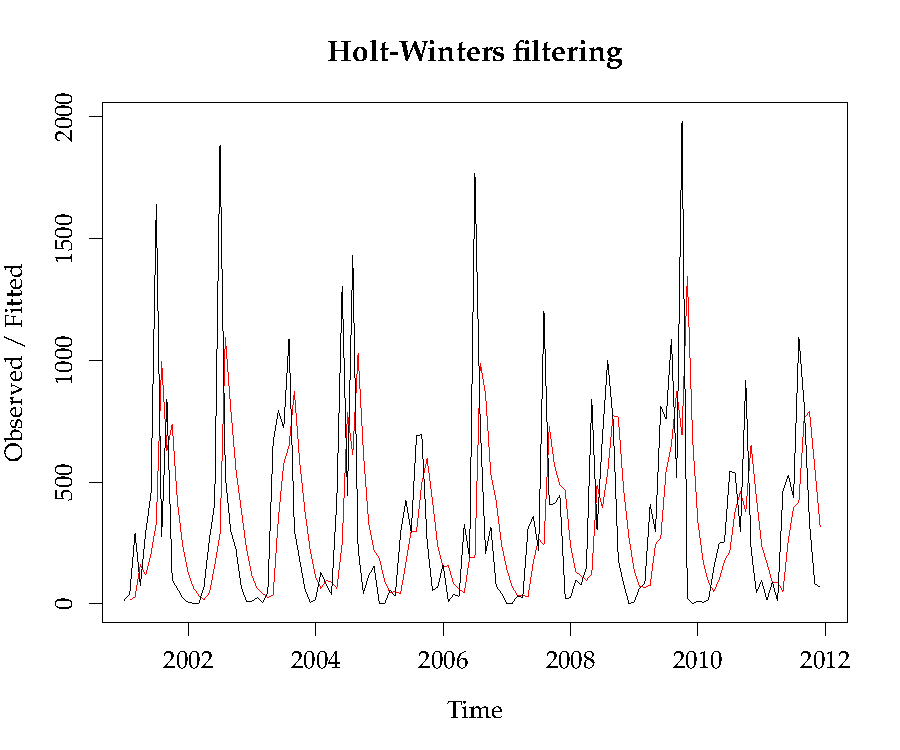
\includegraphics[width=.7\textwidth]{figure/listings-fittedgraph} \end{Schunk}

\caption{\label{fig:fittedgraph} The original rainfall time series with the predicted values in the same period.}
\end{figure}

We now make forecasts for further time points by using the
\texttt{forecast.HoltWinters()} function in the R \texttt{forecast} package. The result is in \eqref{fig:Forecast2}.

\begin{figure}[!ht]
\begin{Schunk}
\begin{Sinput}
library(forecast)
\end{Sinput}
\begin{Soutput}
This is forecast 4.01 
\end{Soutput}
\begin{Sinput}
baguiorainseriesforecasts2 <- forecast.HoltWinters(baguiorainseriesforecasts, 
    h = 12)
baguiorainseriesforecasts2
\end{Sinput}
\begin{Soutput}
         Point Forecast   Lo 80  Hi 80   Lo 95  Hi 95
Jan 2012          59.32 -366.29  484.9 -591.60  710.2
Feb 2012          40.91 -384.70  466.5 -610.01  691.8
Mar 2012          74.48 -351.14  500.1 -576.44  725.4
Apr 2012         132.45 -293.17  558.1 -518.48  783.4
May 2012         417.57   -8.06  843.2 -233.37 1068.5
Jun 2012         486.53   60.90  912.2 -164.42 1137.5
Jul 2012         609.41  183.77 1035.0  -41.56 1260.4
Aug 2012         945.05  519.40 1370.7  294.07 1596.0
Sep 2012         592.75  167.08 1018.4  -58.25 1243.7
Oct 2012         702.69  277.01 1128.4   51.66 1353.7
Nov 2012         142.04 -283.66  567.7 -509.02  793.1
Dec 2012          57.36 -368.37  483.1 -593.73  708.4
\end{Soutput}
\end{Schunk}

\caption{\label{fig:Forecast2} The 12-month forecast for the year 2012 based on \texttt{Holt Winters} smoothing.}
\end{figure}

\begin{figure}[!ht]
\centering
\begin{Schunk}
\begin{Sinput}
plot.forecast(baguiorainseriesforecasts2)
\end{Sinput}

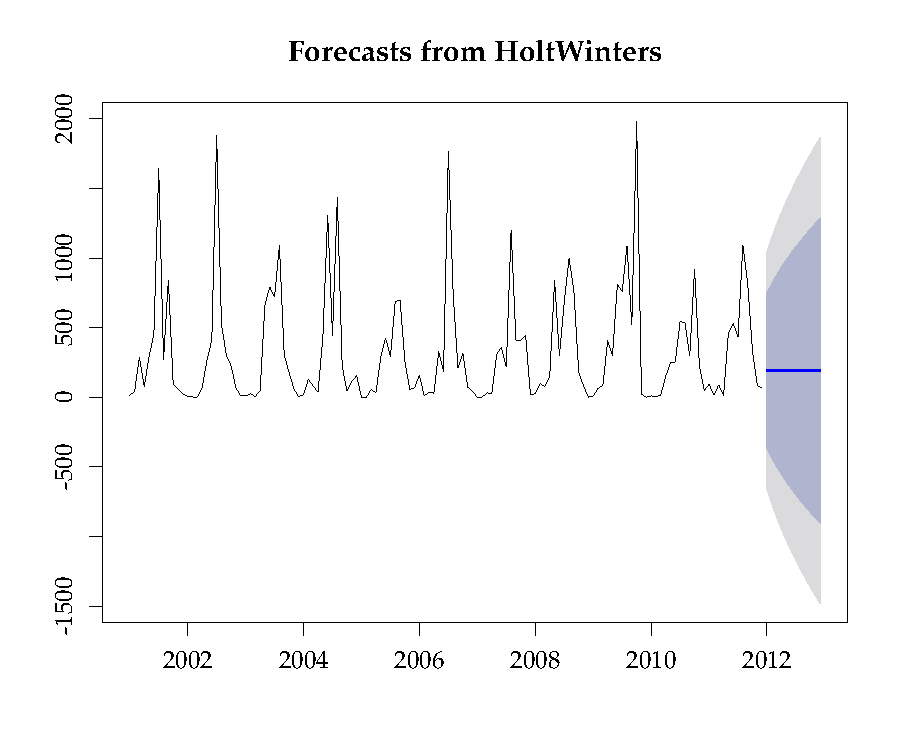
\includegraphics[width=.7\textwidth]{figure/listings-ForecastFigure} \end{Schunk}

\caption{\label{fig:ForecastFigure}Graph of forecast for rainfall time series data.}
\end{figure}

To see if the prediction can be improved, we will use the \texttt{Ljung Box Test} through the \texttt{Box.test()} function.

\begin{Schunk}
\begin{Sinput}
Box.test(baguiorainseriesforecasts2$residuals, lag = 20, type = "Ljung-Box")
\end{Sinput}
\begin{Soutput}

	Box-Ljung test

data:  baguiorainseriesforecasts2$residuals 
X-squared = 23.91, df = 20, p-value = 0.2465
\end{Soutput}
\end{Schunk}


Here, the $p$-value of \num{3.553e-13} tells us that the prediction can be improved. We can remove the \texttt{seasonal} component of the data, save it to an external file and call it back to \textsf{R} as follows.

\begin{Schunk}
\begin{Sinput}
baguiorainseriesseasonallyadjusted <- read.table("baguiorainseriesseasonallyadjusted.dat")
baguiorainseriesseasonallyadjustedts <- ts(baguiorainseriesseasonallyadjusted, 
    frequency = 12, start = c(2001, 1))
\end{Sinput}
\end{Schunk}


Figure \eqref{fig:AdjustedPlot} contains the plot of seasonally adjusted rainfall time series.

\begin{center}
\begin{Schunk}
\begin{Sinput}
plot.ts(baguiorainseriesseasonallyadjustedts)
\end{Sinput}

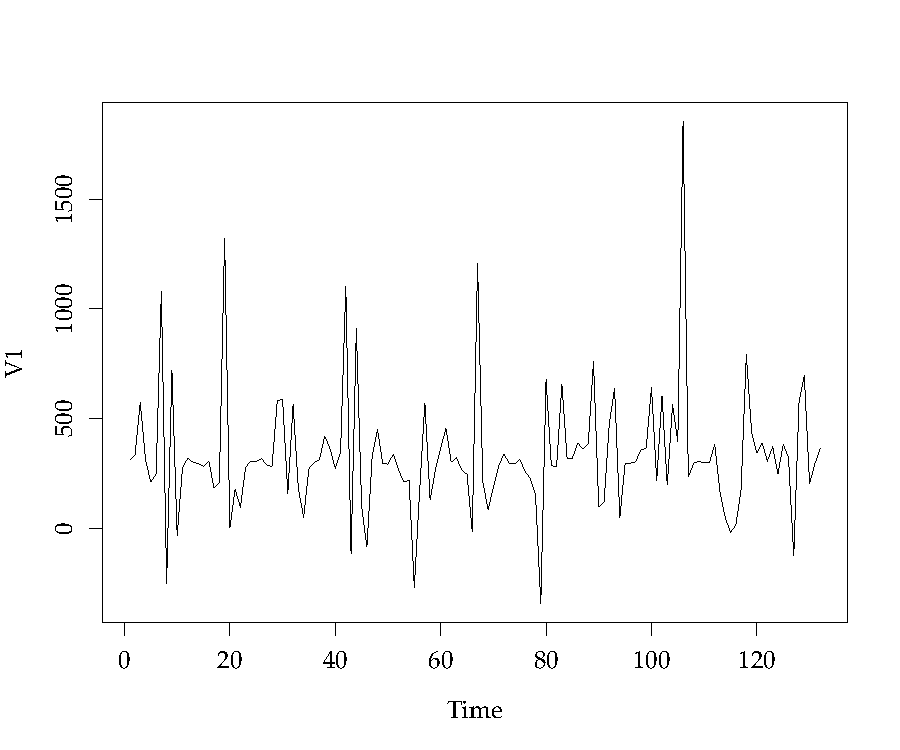
\includegraphics[width=.7\textwidth]{figure/listings-AdjustedPlot} \end{Schunk}

\captionof{figure}{\label{fig:AdjustedPlot}Plot of seasonally adjusted rainfall time series.}
\end{center}

We shall now see if this prediction can still be improved by going through our previous steps.

\begin{Schunk}
\begin{Sinput}
baguiorainseriesseasonallyadjustedtsforecast <- HoltWinters(baguiorainseriesseasonallyadjustedts, 
    beta = FALSE, gamma = FALSE)
baguiorainseriesseasonallyadjustedtsforecast
\end{Sinput}
\begin{Soutput}
Holt-Winters exponential smoothing without trend and without seasonal component.

Call:
 HoltWinters(x = baguiorainseriesseasonallyadjustedts, beta = FALSE,      gamma = FALSE) 

Smoothing parameters:
 alpha:  6.611e-05 
 beta :  FALSE 
 gamma:  FALSE 

Coefficients:
   [,1]
a 311.3
\end{Soutput}
\begin{Sinput}
baguiorainseriesseasonallyadjustedforecastvalue <- forecast.HoltWinters(baguiorainseriesseasonallyadjustedtsforecast, 
    h = 12)
baguiorainseriesseasonallyadjustedforecastvalue
\end{Sinput}
\begin{Soutput}
         Point Forecast  Lo 80 Hi 80  Lo 95 Hi 95
Jan 2012          311.3 -53.89 676.6 -247.2 869.9
Feb 2012          311.3 -53.89 676.6 -247.2 869.9
Mar 2012          311.3 -53.89 676.6 -247.2 869.9
Apr 2012          311.3 -53.89 676.6 -247.2 869.9
May 2012          311.3 -53.89 676.6 -247.2 869.9
Jun 2012          311.3 -53.89 676.6 -247.2 869.9
Jul 2012          311.3 -53.89 676.6 -247.2 869.9
Aug 2012          311.3 -53.89 676.6 -247.2 869.9
Sep 2012          311.3 -53.89 676.6 -247.2 869.9
Oct 2012          311.3 -53.89 676.6 -247.2 869.9
Nov 2012          311.3 -53.89 676.6 -247.2 869.9
Dec 2012          311.3 -53.89 676.6 -247.2 869.9
\end{Soutput}
\begin{Sinput}
predict(baguiorainseriesseasonallyadjustedtsforecast, n.ahead = 12, prediction.interval = TRUE, 
    level = 0.95)
\end{Sinput}
\begin{Soutput}
           fit   upr    lwr
Jan 2012 311.3 869.9 -247.2
Feb 2012 311.3 869.9 -247.2
Mar 2012 311.3 869.9 -247.2
Apr 2012 311.3 869.9 -247.2
May 2012 311.3 869.9 -247.2
Jun 2012 311.3 869.9 -247.2
Jul 2012 311.3 869.9 -247.2
Aug 2012 311.3 869.9 -247.2
Sep 2012 311.3 869.9 -247.2
Oct 2012 311.3 869.9 -247.2
Nov 2012 311.3 869.9 -247.2
Dec 2012 311.3 869.9 -247.2
\end{Soutput}
\begin{Sinput}
prediction <- predict(baguiorainseriesseasonallyadjustedtsforecast, n.ahead = 12, 
    prediction.interval = TRUE, level = 0.95)
\end{Sinput}
\end{Schunk}


\begin{center}
\begin{Schunk}
\begin{Sinput}
plot.forecast(baguiorainseriesseasonallyadjustedforecastvalue)
\end{Sinput}

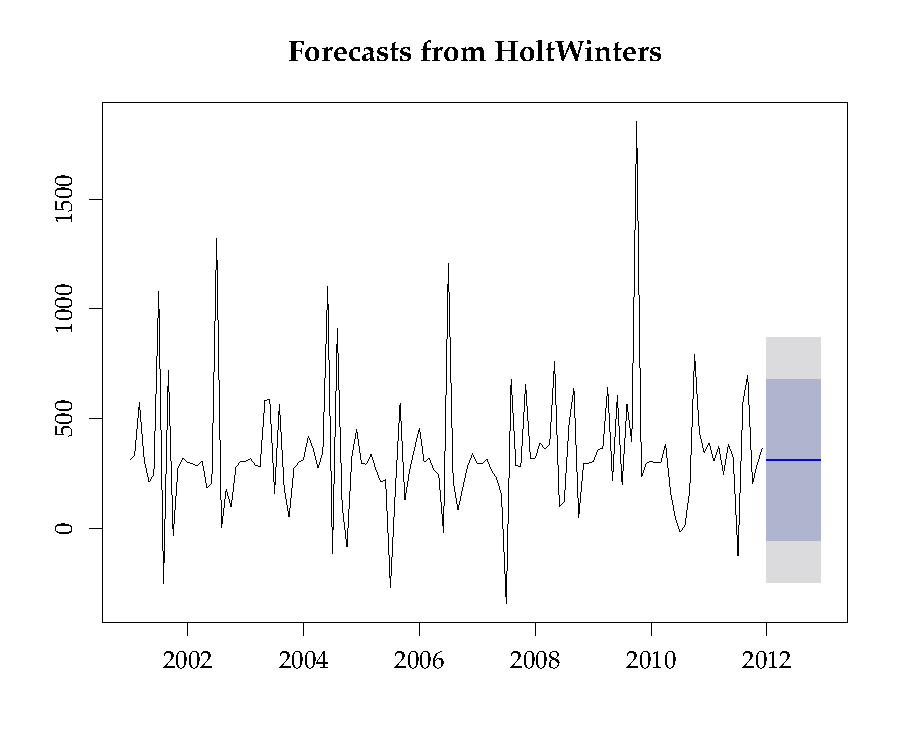
\includegraphics[width=.7\textwidth]{figure/listings-ForecastAdjusted} \end{Schunk}

\captionof{figure}{\label{fig:ForecastAdjusted} Graph of forecast for seasonally-adjusted rainfall time series.}
\end{center}

The $\alpha$ value of \num{6.611 e -05} is very close to zero, telling us that the forecasts are based on both recent and less recent observations.

\section{Summary of \texttt{R} code used in this document}
\begin{listing}[!ht]
\begin{Schunk}
\begin{Sinput}
baguiorain <- read.table("baguiorainfall.dat")
baguiorainseries <- ts(baguiorain, frequency = 12, start = c(2001, 1))
plot.ts(baguiorainseries)
baguiorainseriescomponents <- decompose(baguiorainseries)
baguiorainseriescomponents
plot(baguiorainseriescomponents)
baguiorainseriesforecasts <- HoltWinters(baguiorainseries, beta = FALSE, gamma = FALSE)
baguiorainseriesforecasts
baguiorainseriesforecasts$fitted
plot(baguiorainseriesforecasts)
library(forecast)
baguiorainseriesforecasts2 <- forecast.HoltWinters(baguiorainseriesforecasts, 
    h = 12)
baguiorainseriesforecasts2
plot.forecast(baguiorainseriesforecasts2)
Box.test(baguiorainseriesforecasts2$residuals, lag = 20, type = "Ljung-Box")
baguiorainseriesseasonallyadjusted <- read.table("baguiorainseriesseasonallyadjusted.dat")
baguiorainseriesseasonallyadjustedts <- ts(baguiorainseriesseasonallyadjusted, 
    frequency = 12, start = c(2001, 1))
plot.ts(baguiorainseriesseasonallyadjustedts)
baguiorainseriesseasonallyadjustedtsforecast <- HoltWinters(baguiorainseriesseasonallyadjustedts, 
    beta = FALSE, gamma = FALSE)
baguiorainseriesseasonallyadjustedtsforecast
baguiorainseriesseasonallyadjustedforecastvalue <- forecast.HoltWinters(baguiorainseriesseasonallyadjustedtsforecast, 
    h = 12)
baguiorainseriesseasonallyadjustedforecastvalue
predict(baguiorainseriesseasonallyadjustedtsforecast, n.ahead = 12, prediction.interval = TRUE, 
    level = 0.95)
prediction <- predict(baguiorainseriesseasonallyadjustedtsforecast, n.ahead = 12, 
    prediction.interval = TRUE, level = 0.95)
plot.forecast(baguiorainseriesseasonallyadjustedforecastvalue)
\end{Sinput}
\end{Schunk}

\caption{\label{list:listingsummary} Summary of \texttt{R} codes used.}
\end{listing}

\begin{Schunk}
\begin{Sinput}
Data2012 <- c(17.5, 80.3, 151.9, 72, 207.7, 659, 1020.2, 2207, 288.3, 72.4, 
    57.8, 10.8)
Forecastval <- c(190.3, 190.3, 190.3, 190.3, 190.3, 190.3, 190.3, 190.3, 190.3, 
    190.3, 190.3, 190.3)
Forecastval2 <- c(311.3, 311.3, 311.3, 311.3, 311.3, 311.3, 311.3, 311.3, 311.3, 
    311.3, 311.3, 311.3)
TTestData1 <- data.frame(Data2012, Forecastval, Forecastval2)
attach(TTestData1)
\end{Sinput}
\begin{Soutput}
The following object(s) are masked _by_ '.GlobalEnv':

    Data2012, Forecastval, Forecastval2
\end{Soutput}
\begin{Sinput}
t.test(Data2012, Forecastval)
\end{Sinput}
\begin{Soutput}

	Welch Two Sample t-test

data:  Data2012 and Forecastval 
t = 1.148, df = 11, p-value = 0.2752
alternative hypothesis: true difference in means is not equal to 0 
95 percent confidence interval:
 -195.6  622.5 
sample estimates:
mean of x mean of y 
    403.7     190.3 
\end{Soutput}
\begin{Sinput}
t.test(Data2012, Forecastval2)
\end{Sinput}
\begin{Soutput}

	Welch Two Sample t-test

data:  Data2012 and Forecastval2 
t = 0.4974, df = 11, p-value = 0.6287
alternative hypothesis: true difference in means is not equal to 0 
95 percent confidence interval:
 -316.6  501.5 
sample estimates:
mean of x mean of y 
    403.7     311.3 
\end{Soutput}
\end{Schunk}


\end{document}
